%
% $RCSfile: model_transition.tex,v $
%
% Copyright (C) 2002-2008. Christian Heller.
%
% Permission is granted to copy, distribute and/or modify this document
% under the terms of the GNU Free Documentation License, Version 1.1 or
% any later version published by the Free Software Foundation; with no
% Invariant Sections, with no Front-Cover Texts and with no Back-Cover
% Texts. A copy of the license is included in the section entitled
% "GNU Free Documentation License".
%
% http://www.cybop.net
% - Cybernetics Oriented Programming -
%
% http://www.resmedicinae.org
% - Information in Medicine -
%
% Version: $Revision: 1.1 $ $Date: 2008-08-19 20:41:07 $ $Author: christian $
% Authors: Christian Heller <christian.heller@tuxtax.de>
%

\subsection{Model Transition}
\label{model_transition_heading}
\index{CYBOI Model Transition}
\index{Knowledge Template}
\index{Knowledge Model}
\index{Information Processing Model}
\index{CYBOI as Universal Data Converter}

The creation of transient knowledge models (to be kept in memory, at runtime)
from persistent knowledge templates (given in form of CYBOL sources) is not a
trivial thing. It is a mechanism consisting of a cascade of model transitions,
comparable to the \emph{Information Processing Model} of cognitive psychology
(section \ref{information_processing_model_heading}). One may imagine this as a
state changing its appearance, while \emph{wandering} through the system. The
same mechanism is applied when handling communication data (figure
\ref{transition_figure}). Because CYBOI's architecture is easily extensible
with various modules, such as \emph{import/ export} (i/e) filters for different
kinds of communication, it may act as universal data converter. All
corresponding modules belong to the \emph{Memoriser} part of CYBOI.

\begin{figure}[ht]
    \begin{center}
        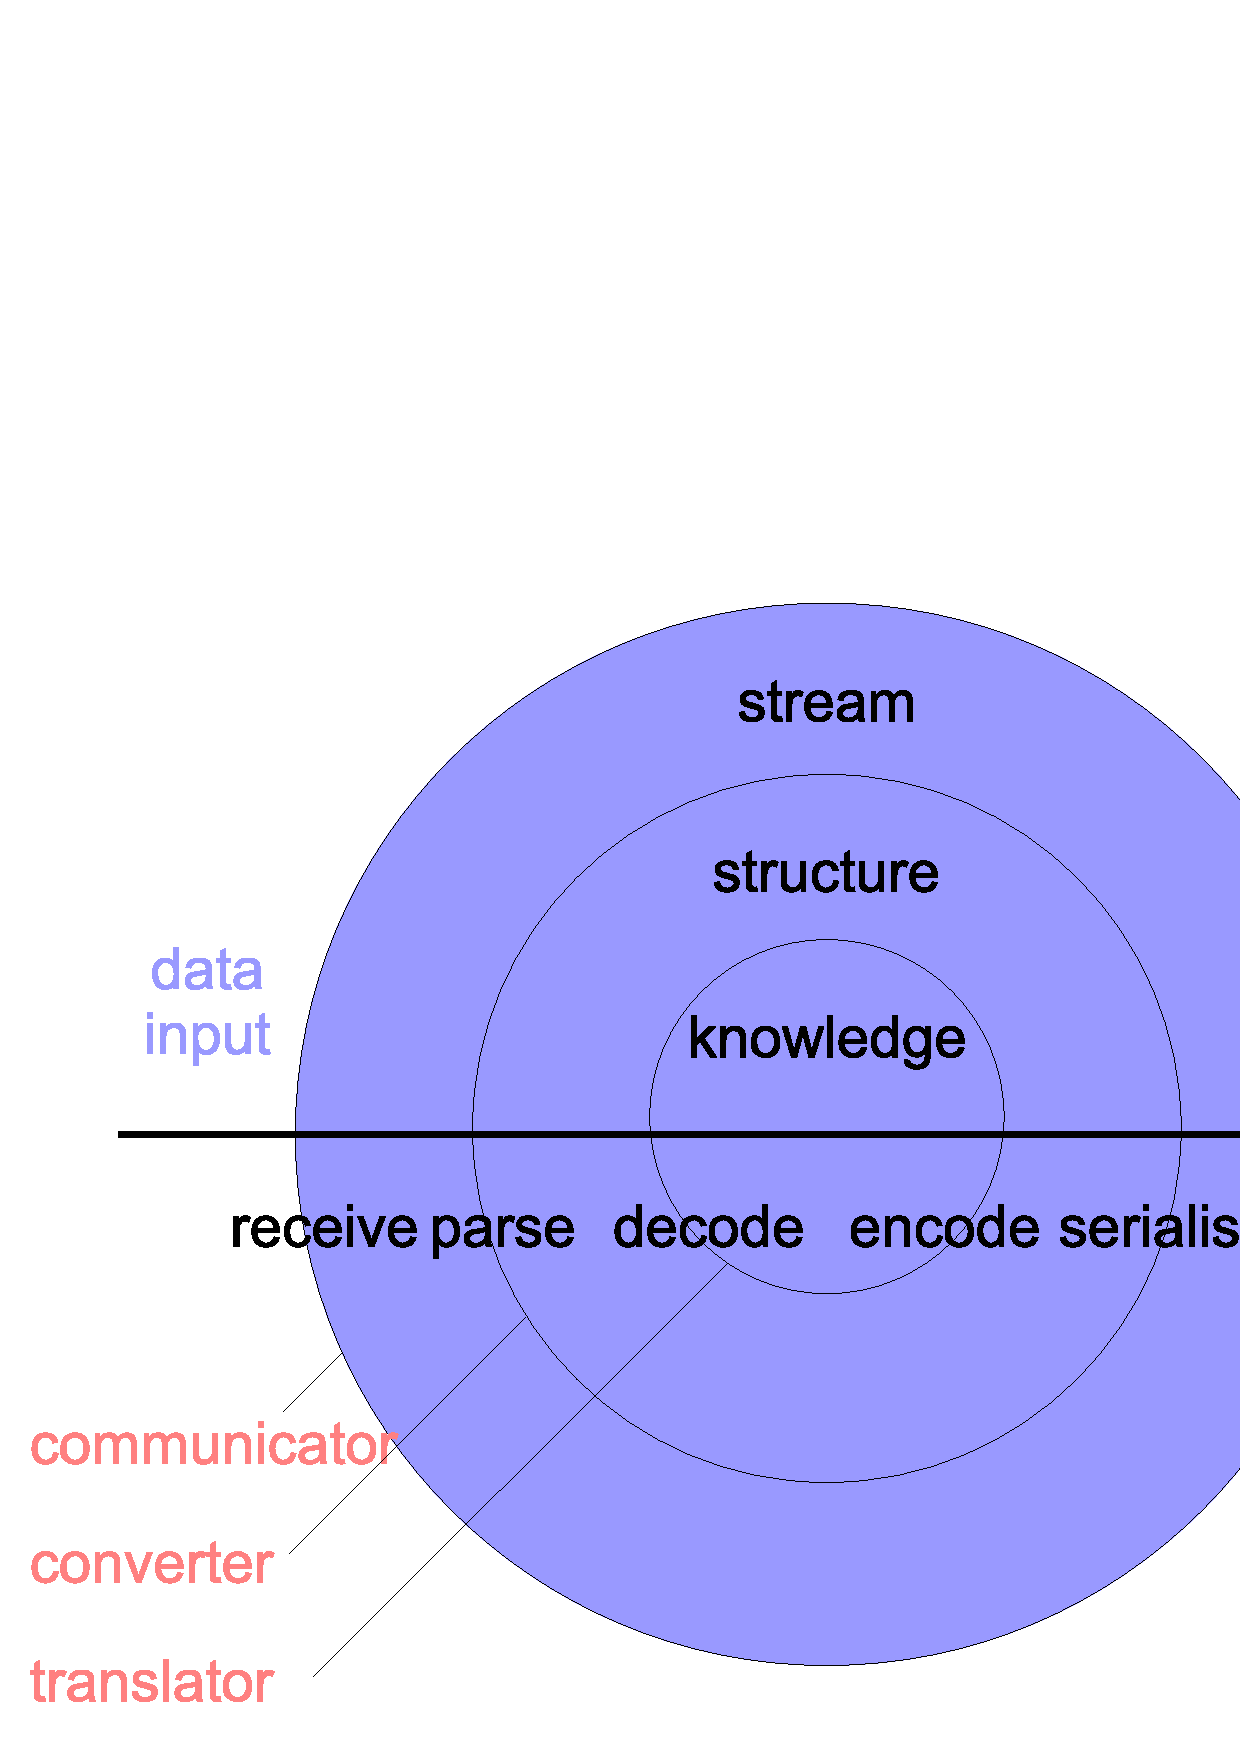
\includegraphics[scale=0.3,angle=-90]{graphic/transition.pdf}
        \caption{Input-to-Output Model Transition}
        \label{transition_figure}
    \end{center}
\end{figure}

As opposed to the knowledge acquirement in \emph{Artificial Neural Networks}
(ANN),
%(section \ref{artificial_neural_network_heading}),
the knowledge in CYBOP
systems is not learned, but \emph{injected} by reading from external knowledge
sources, which can be manipulated in a flexible manner any time. The difference
to standard applications is that these hard-wire their knowledge within the
system.

A data input (i/p), after having been processed by a \emph{receive} procedure
(\emph{communicator} modules), results in a stream -- a data array in memory. A
\emph{parse} procedure (\emph{converter} modules), depending on the kind of
abstraction of the data, then builds a structure out of this simple array. The
structure, finally, passes a \emph{decode} procedure (\emph{translator}
modules) which creates a knowledge model.

Whenever an application running within CYBOI wants to send data, may it be to
another system or for making them persistent on a local \emph{Hard Disk Drive}
(HDD), translator, converter and communicator have to be crossed in the
opposite direction. Because a running application system is a tree of knowledge
models allocating space in memory, parts of that tree can be \emph{serialised}
easily. It has to be mentioned, though, that slight changes of the XML format
are necessary to achieve this: The usual quotation marks used to delimit XML
attribute values have to be replaced with differing \emph{begin} and \emph{end}
characters. This feature is an open issue which the current version of CYBOI
does not provide yet.

%Isn't CYBOI model transition similar to termios Zeichenverarbeitung in Linux?
%siehe Grafik im Buch: Anwendungen entwickeln unter Linux, S. 249
